\documentclass[11pt]{article}
\usepackage[textwidth=18.0cm, textheight=23.0cm, top=2.0cm]{geometry}
\usepackage{pst-all}
\usepackage{amssymb}
\usepackage{tikz}
\usepackage{underscore}\begin{document}
\pagestyle{empty}


ClassName: \underline{\textbf{Class_08.2bp-13}}
\par
BinSize: \underline{\textbf{100 × 100}}
\par
ReduceSize: \underline{\textbf{100 × 100}}
\par
TypeNum: \underline{\textbf{40}}
\par
Num: \underline{\textbf{40}}
\par
OutS: \underline{\textbf{120000}}
\par
InS: \underline{\textbf{99739}}
\par
Rate: \underline{\textbf{0.831}}
\par
UB: \underline{\textbf{12}}
\par
LB0: \underline{\textbf{12}}
\par
LB: \underline{\textbf{12}}
\par
LBWithCut: \underline{\textbf{12}}
\par
NodeCut: \underline{\textbf{0}}
\par
ExtendedNodeCnt: \underline{\textbf{1}}
\par
GenNodeCnt: \underline{\textbf{1}}
\par
PrimalNode: \underline{\textbf{0}}
\par
ColumnCount: \underline{\textbf{12}}
\par
TotalCutCount: \underline{\textbf{0}}
\par
RootCutCount: \underline{\textbf{0}}
\par
LPSolverCnt: \underline{\textbf{1}}
\par
PricingSolverCnt: \underline{\textbf{0}}
\par
BranchAndBoundNum: \underline{\textbf{1}}
\par
isOpt: \underline{\textbf{true}}
\par
TimeOnInitSolution: \underline{\textbf{600.000 s}}
\par
TimeOnPrimal: \underline{\textbf{0.000 s}}
\par
TimeOnPricing: \underline{\textbf{0.000 s}}
\par
TimeOnRmp: \underline{\textbf{0.063 s}}
\par
TotalTime: \underline{\textbf{600.297 s}}
\par
\newpage


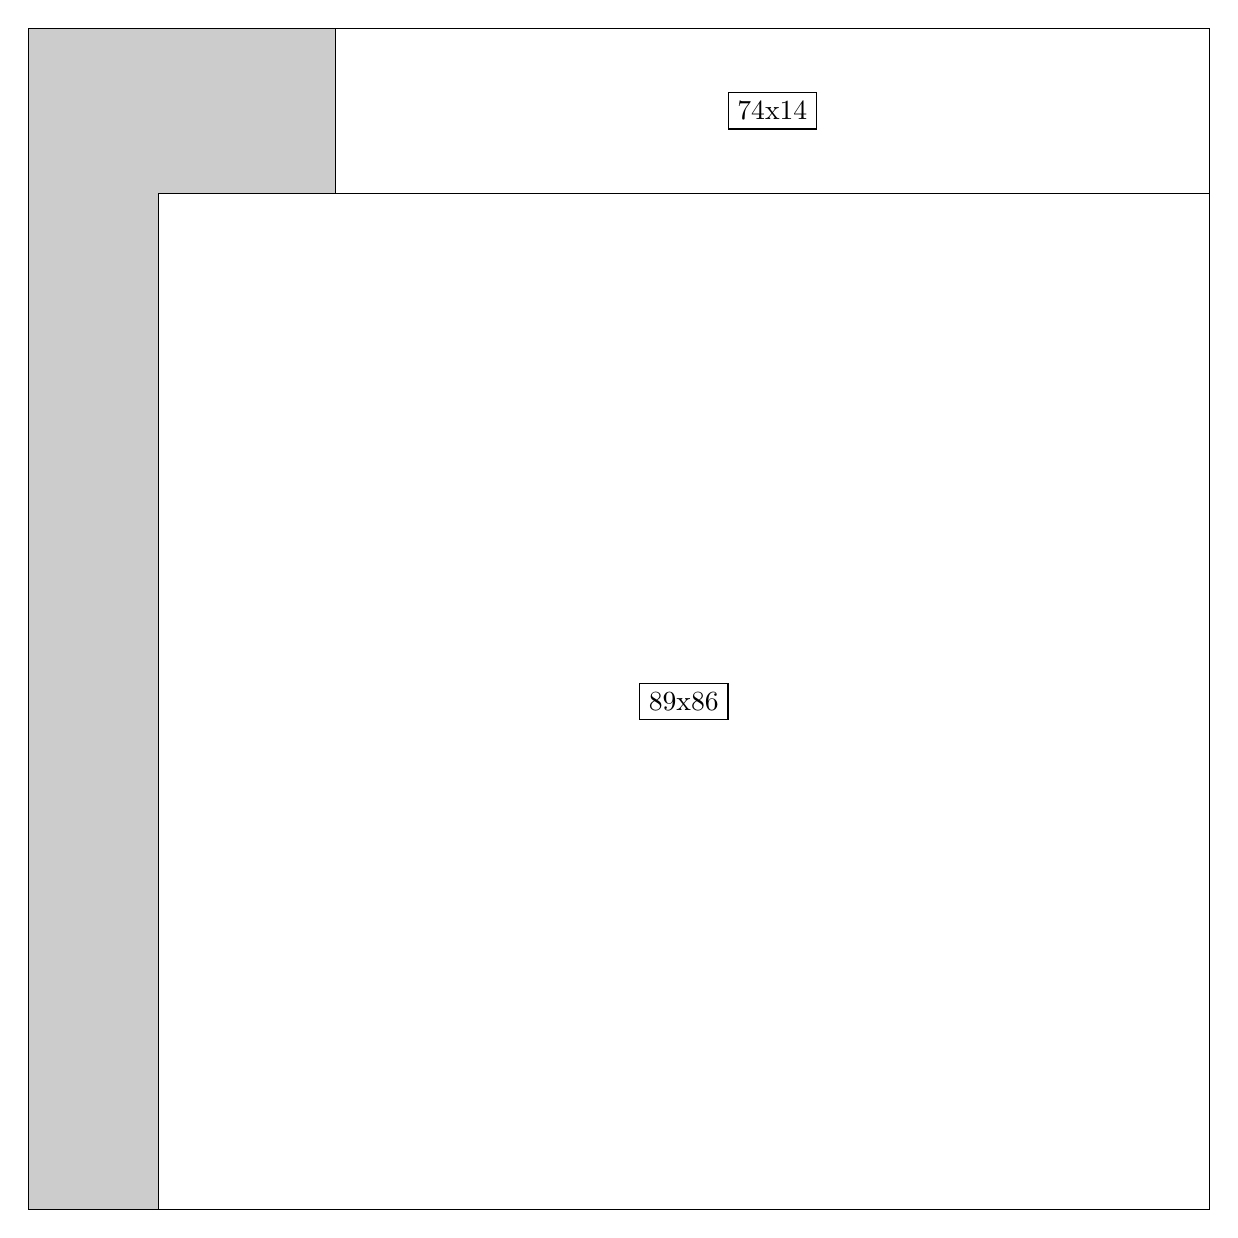
\begin{tikzpicture}[shorten >=1pt,scale=1.0,every node/.style={scale=1.0},->]
\tikzstyle{vertex}=[circle,fill=black!25,minimum size=14pt,inner sep=0pt]
\filldraw[fill=gray!40!white, draw=black] (0,0) rectangle (15.0,15.0);
\foreach \name/\x/\y/\w/\h in {89x86/1.65/0.0/13.35/12.9,74x14/3.9/12.9/11.1/2.1}
\filldraw[fill=white!40!white, draw=black] (\x,\y) rectangle node[draw] (\name) {\name} ++(\w,\h);
\end{tikzpicture}


w =89 , h =86 , x =11 , y =0 , v =7654
\par
w =74 , h =14 , x =26 , y =86 , v =1036
\par
\newpage


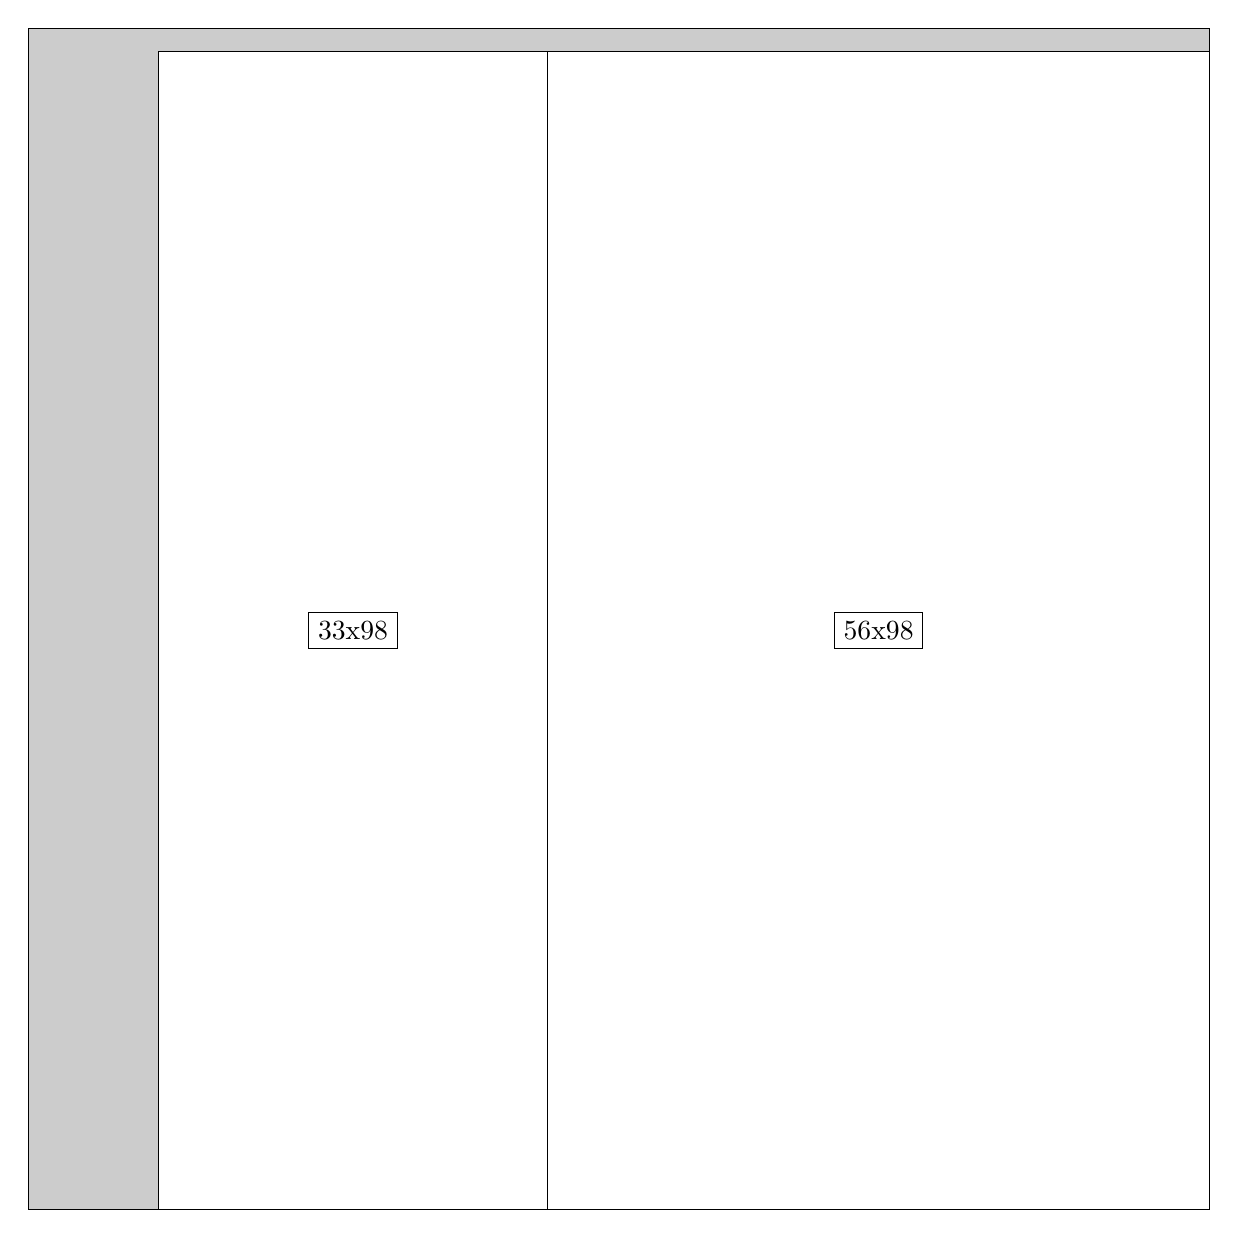
\begin{tikzpicture}[shorten >=1pt,scale=1.0,every node/.style={scale=1.0},->]
\tikzstyle{vertex}=[circle,fill=black!25,minimum size=14pt,inner sep=0pt]
\filldraw[fill=gray!40!white, draw=black] (0,0) rectangle (15.0,15.0);
\foreach \name/\x/\y/\w/\h in {56x98/6.6/0.0/8.4/14.7,33x98/1.65/0.0/4.95/14.7}
\filldraw[fill=white!40!white, draw=black] (\x,\y) rectangle node[draw] (\name) {\name} ++(\w,\h);
\end{tikzpicture}


w =56 , h =98 , x =44 , y =0 , v =5488
\par
w =33 , h =98 , x =11 , y =0 , v =3234
\par
\newpage


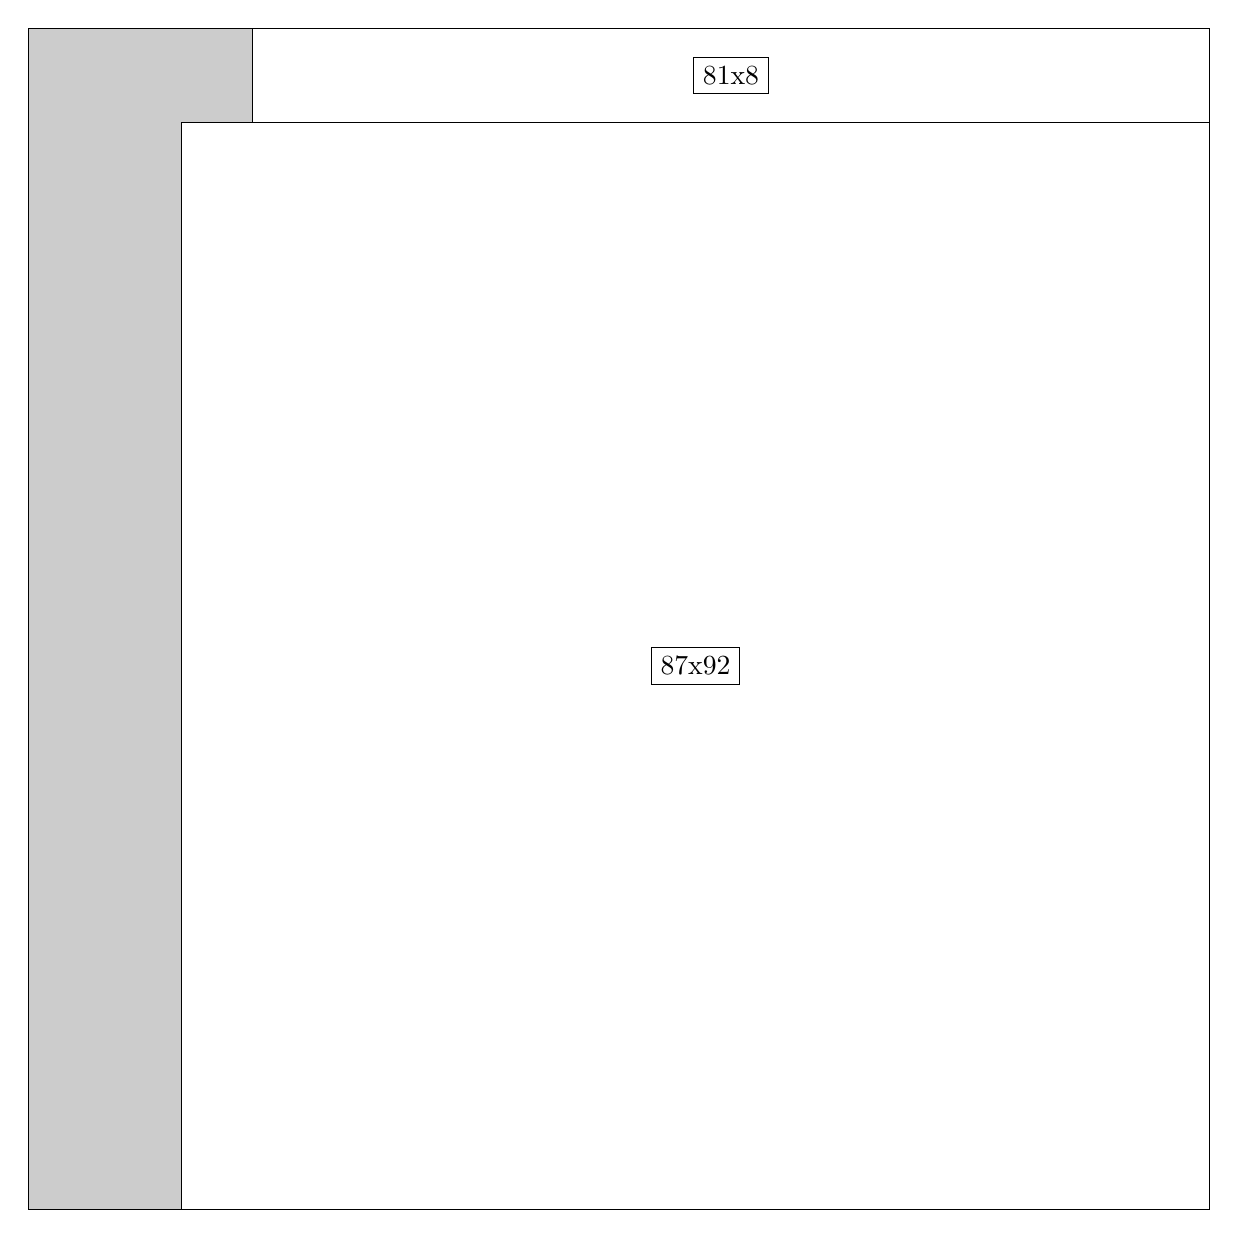
\begin{tikzpicture}[shorten >=1pt,scale=1.0,every node/.style={scale=1.0},->]
\tikzstyle{vertex}=[circle,fill=black!25,minimum size=14pt,inner sep=0pt]
\filldraw[fill=gray!40!white, draw=black] (0,0) rectangle (15.0,15.0);
\foreach \name/\x/\y/\w/\h in {87x92/1.95/0.0/13.049999999999999/13.799999999999999,81x8/2.85/13.799999999999999/12.15/1.2}
\filldraw[fill=white!40!white, draw=black] (\x,\y) rectangle node[draw] (\name) {\name} ++(\w,\h);
\end{tikzpicture}


w =87 , h =92 , x =13 , y =0 , v =8004
\par
w =81 , h =8 , x =19 , y =92 , v =648
\par
\newpage



\begin{tikzpicture}[shorten >=1pt,scale=1.0,every node/.style={scale=1.0},->]
\tikzstyle{vertex}=[circle,fill=black!25,minimum size=14pt,inner sep=0pt]
\filldraw[fill=gray!40!white, draw=black] (0,0) rectangle (15.0,15.0);
\foreach \name/\x/\y/\w/\h in {99x97/0.15/0.0/14.85/14.549999999999999}
\filldraw[fill=white!40!white, draw=black] (\x,\y) rectangle node[draw] (\name) {\name} ++(\w,\h);
\end{tikzpicture}


w =99 , h =97 , x =1 , y =0 , v =9603
\par
\newpage


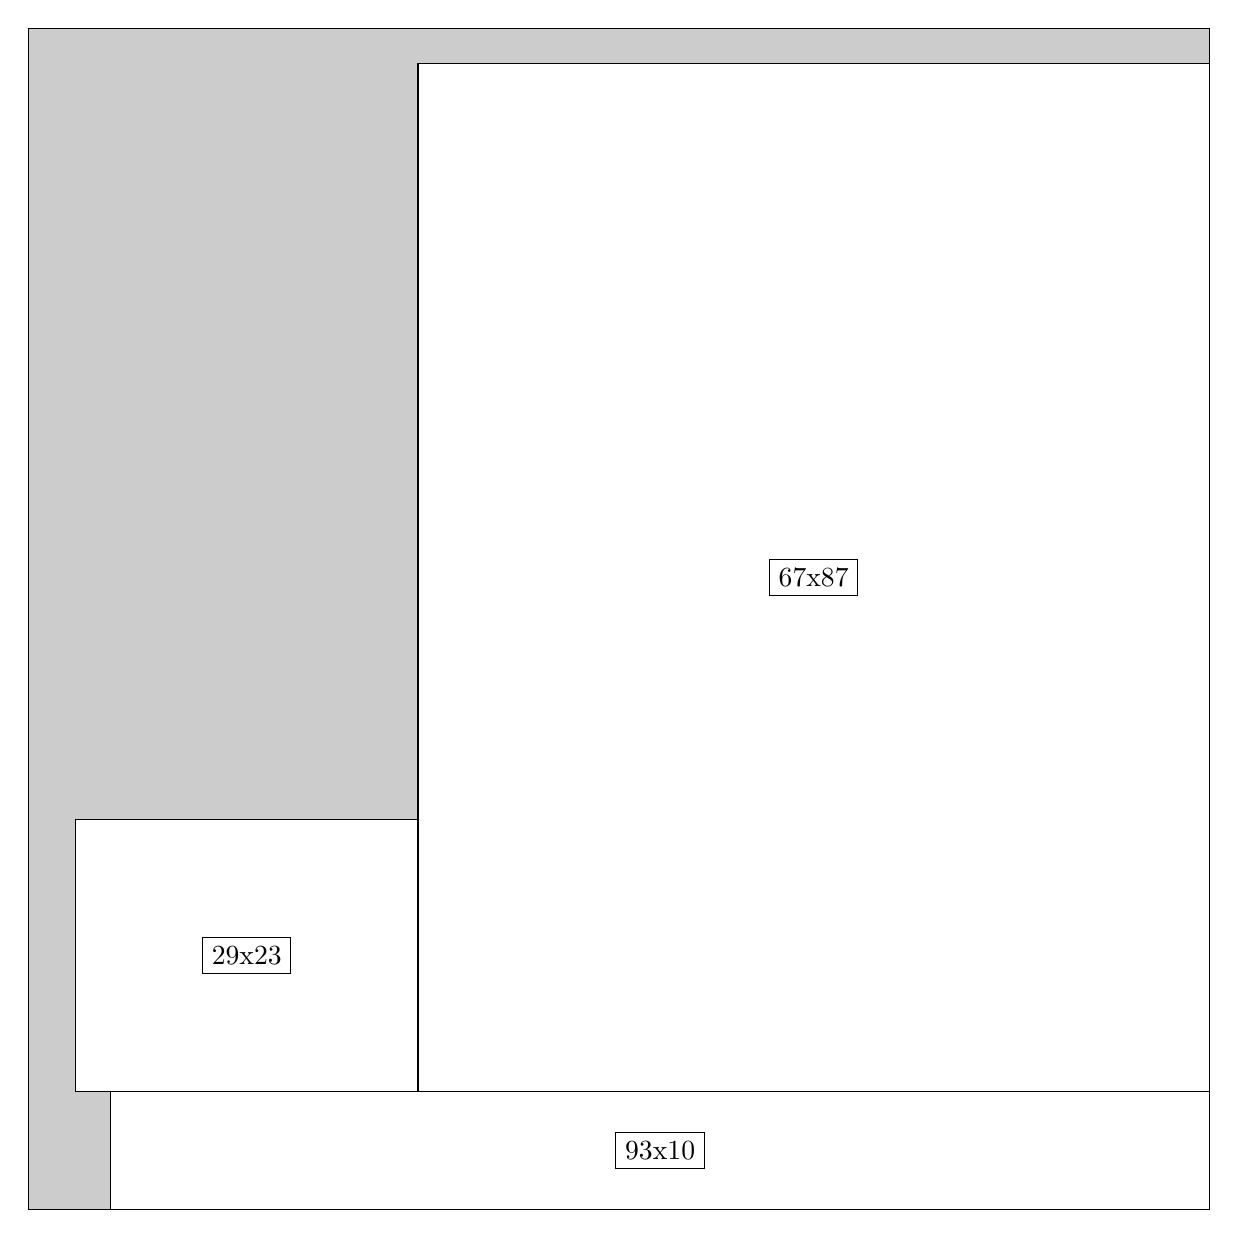
\begin{tikzpicture}[shorten >=1pt,scale=1.0,every node/.style={scale=1.0},->]
\tikzstyle{vertex}=[circle,fill=black!25,minimum size=14pt,inner sep=0pt]
\filldraw[fill=gray!40!white, draw=black] (0,0) rectangle (15.0,15.0);
\foreach \name/\x/\y/\w/\h in {93x10/1.05/0.0/13.95/1.5,67x87/4.95/1.5/10.049999999999999/13.049999999999999,29x23/0.6/1.5/4.35/3.4499999999999997}
\filldraw[fill=white!40!white, draw=black] (\x,\y) rectangle node[draw] (\name) {\name} ++(\w,\h);
\end{tikzpicture}


w =93 , h =10 , x =7 , y =0 , v =930
\par
w =67 , h =87 , x =33 , y =10 , v =5829
\par
w =29 , h =23 , x =4 , y =10 , v =667
\par
\newpage


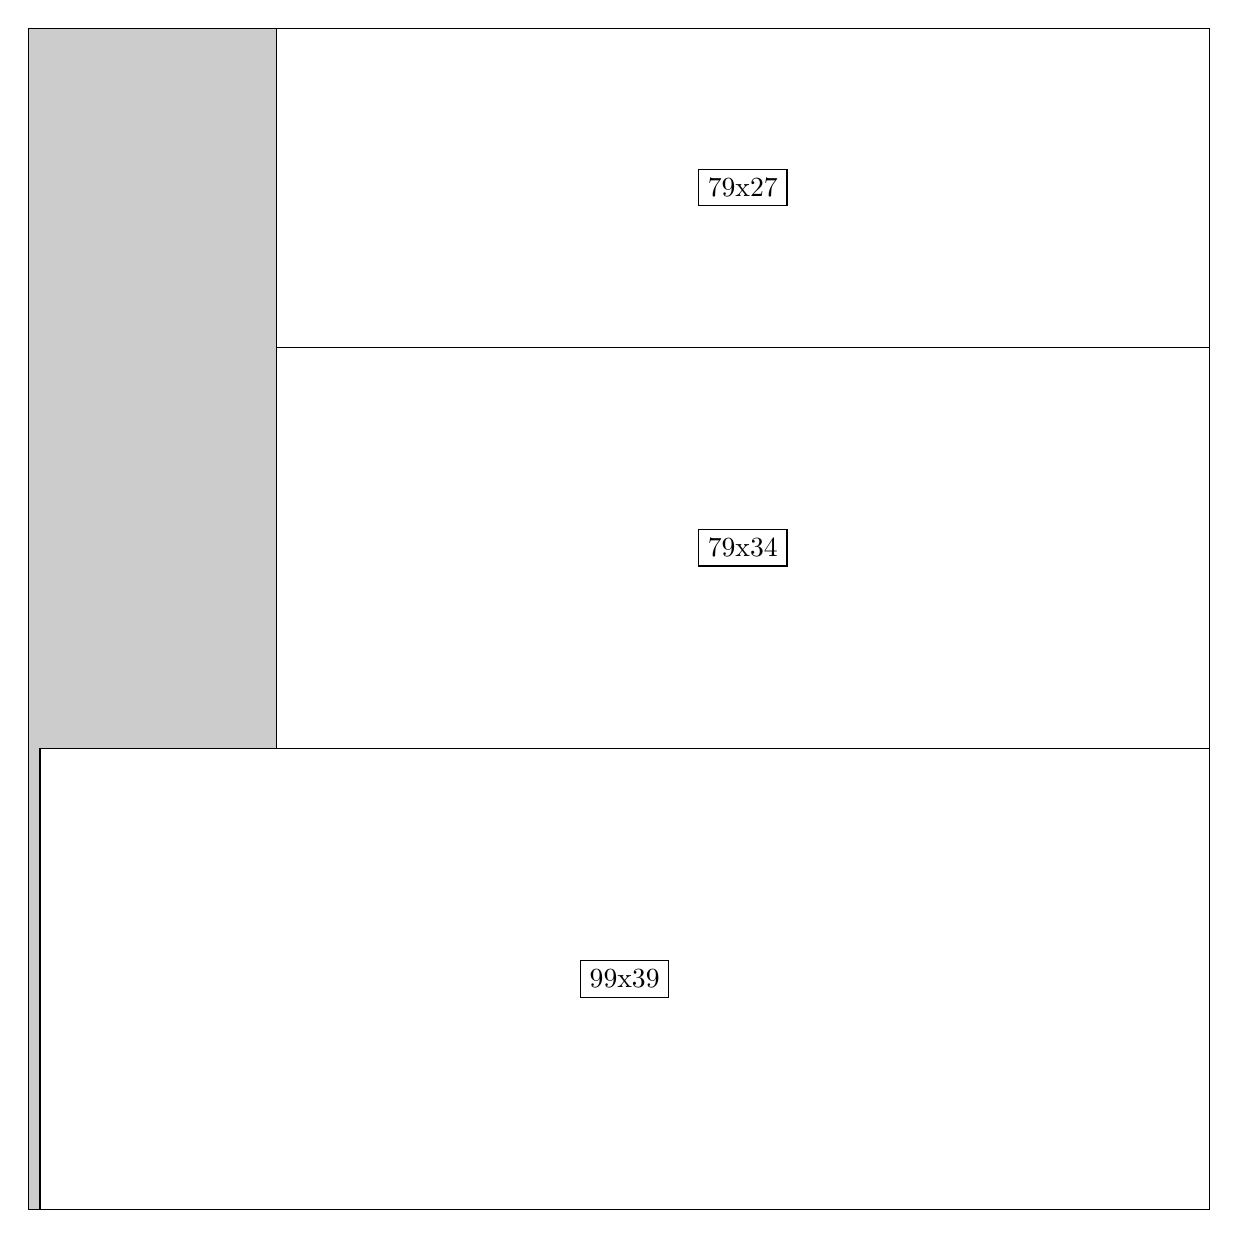
\begin{tikzpicture}[shorten >=1pt,scale=1.0,every node/.style={scale=1.0},->]
\tikzstyle{vertex}=[circle,fill=black!25,minimum size=14pt,inner sep=0pt]
\filldraw[fill=gray!40!white, draw=black] (0,0) rectangle (15.0,15.0);
\foreach \name/\x/\y/\w/\h in {99x39/0.15/0.0/14.85/5.85,79x34/3.15/5.85/11.85/5.1,79x27/3.15/10.95/11.85/4.05}
\filldraw[fill=white!40!white, draw=black] (\x,\y) rectangle node[draw] (\name) {\name} ++(\w,\h);
\end{tikzpicture}


w =99 , h =39 , x =1 , y =0 , v =3861
\par
w =79 , h =34 , x =21 , y =39 , v =2686
\par
w =79 , h =27 , x =21 , y =73 , v =2133
\par
\newpage


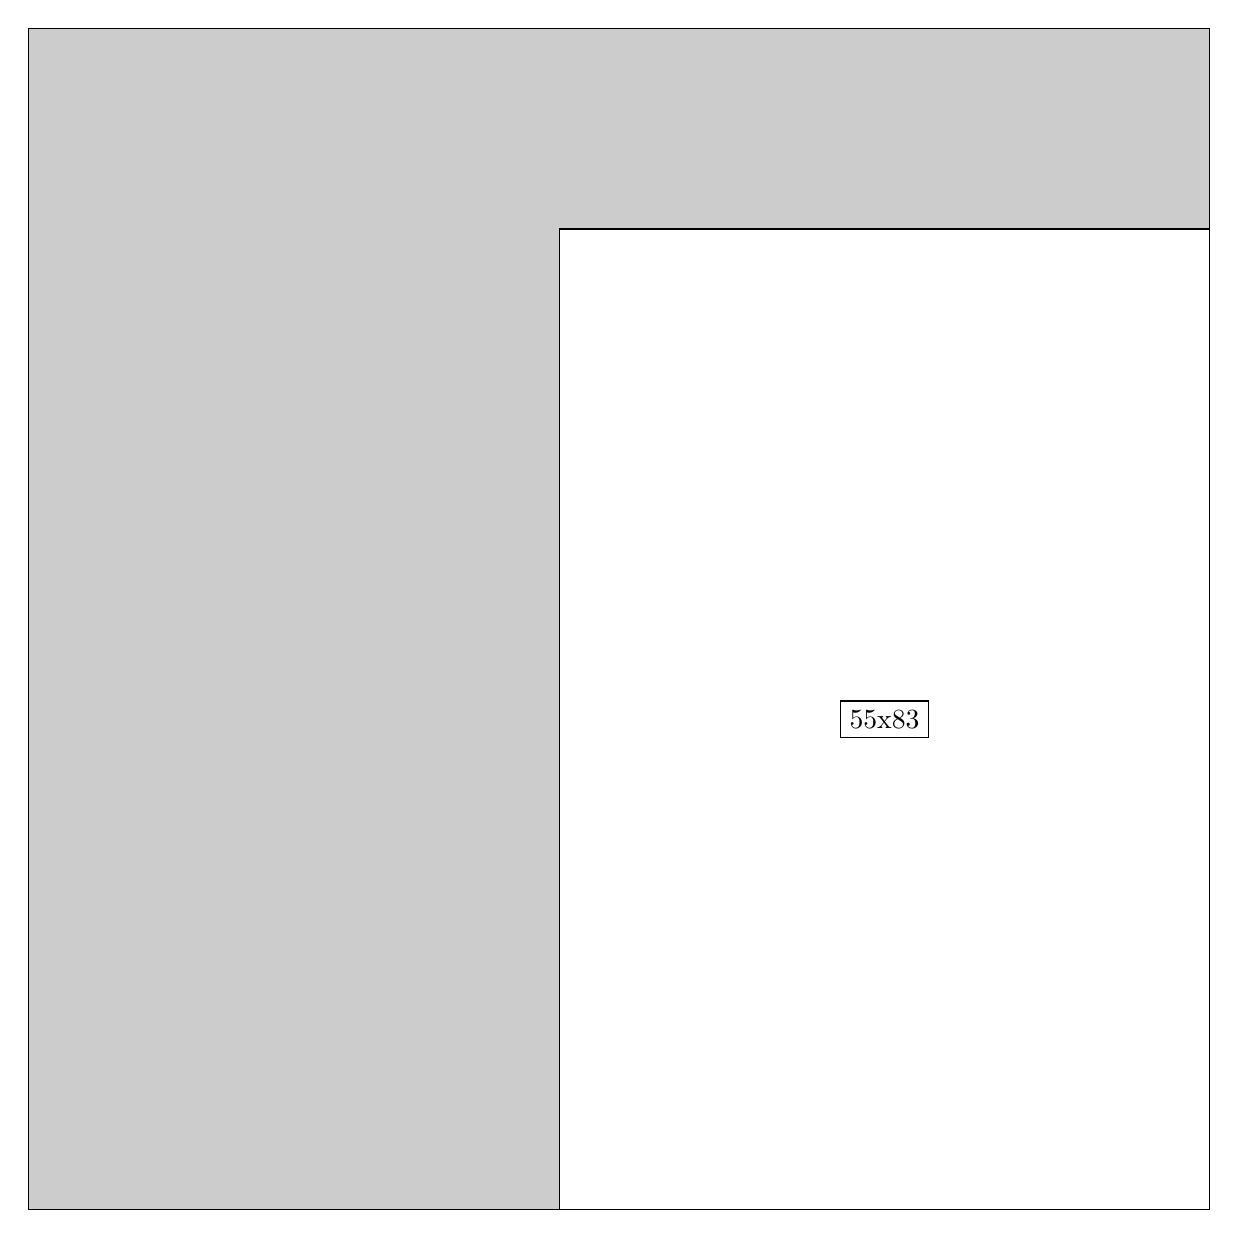
\begin{tikzpicture}[shorten >=1pt,scale=1.0,every node/.style={scale=1.0},->]
\tikzstyle{vertex}=[circle,fill=black!25,minimum size=14pt,inner sep=0pt]
\filldraw[fill=gray!40!white, draw=black] (0,0) rectangle (15.0,15.0);
\foreach \name/\x/\y/\w/\h in {55x83/6.75/0.0/8.25/12.45}
\filldraw[fill=white!40!white, draw=black] (\x,\y) rectangle node[draw] (\name) {\name} ++(\w,\h);
\end{tikzpicture}


w =55 , h =83 , x =45 , y =0 , v =4565
\par
\newpage


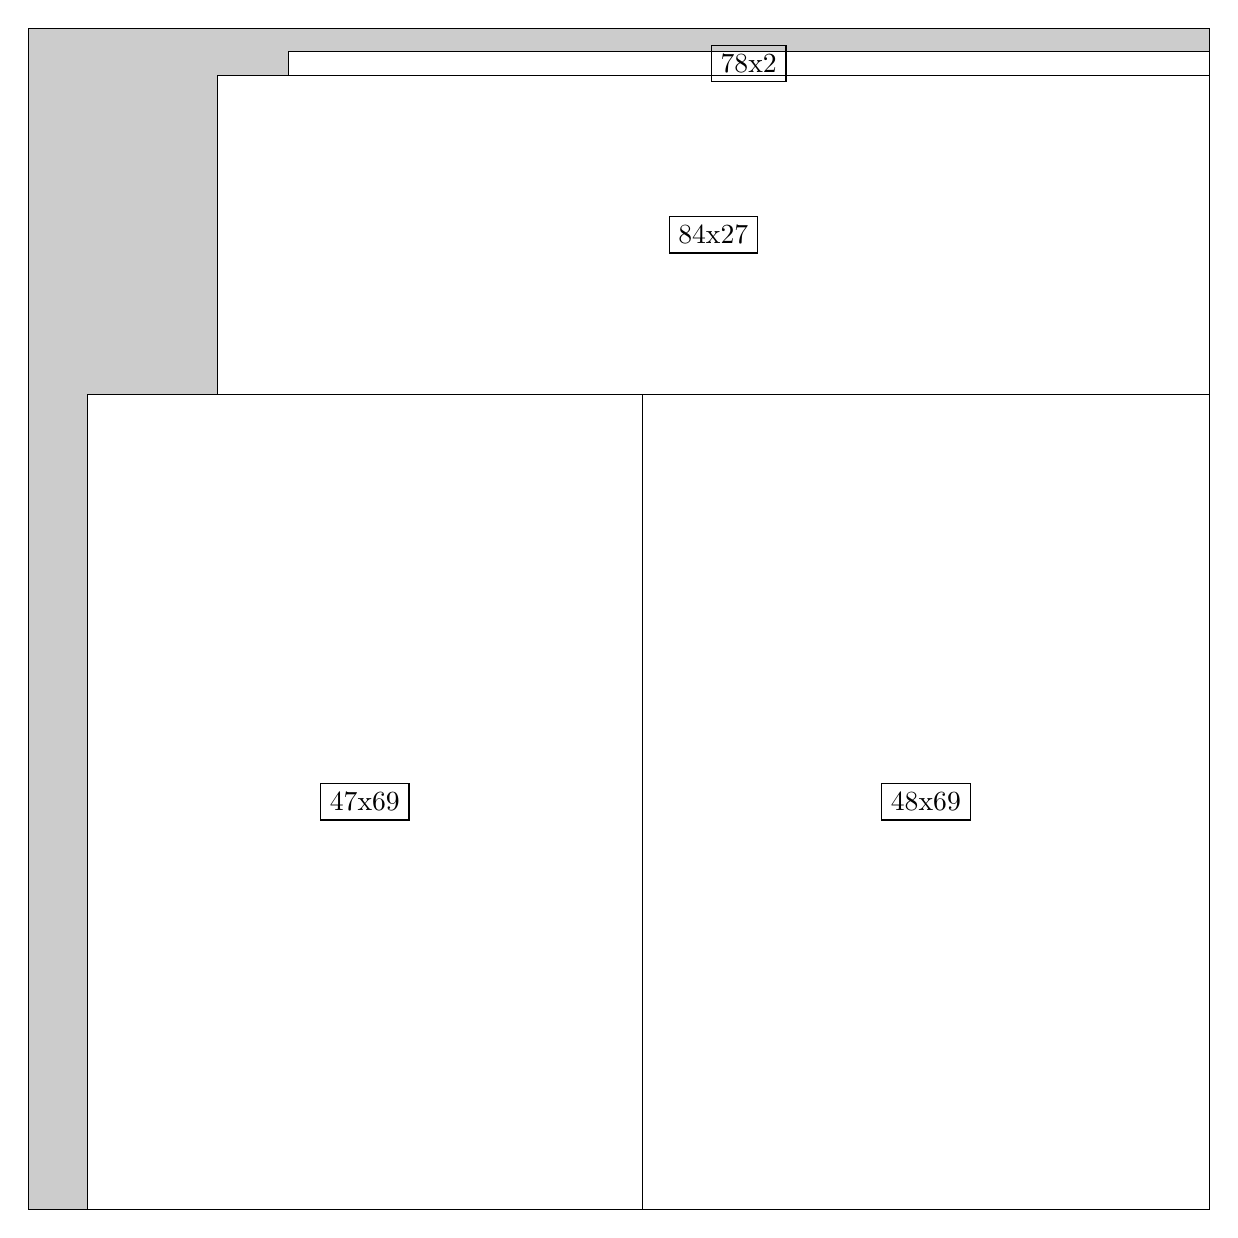
\begin{tikzpicture}[shorten >=1pt,scale=1.0,every node/.style={scale=1.0},->]
\tikzstyle{vertex}=[circle,fill=black!25,minimum size=14pt,inner sep=0pt]
\filldraw[fill=gray!40!white, draw=black] (0,0) rectangle (15.0,15.0);
\foreach \name/\x/\y/\w/\h in {48x69/7.8/0.0/7.199999999999999/10.35,47x69/0.75/0.0/7.05/10.35,84x27/2.4/10.35/12.6/4.05,78x2/3.3/14.399999999999999/11.7/0.3}
\filldraw[fill=white!40!white, draw=black] (\x,\y) rectangle node[draw] (\name) {\name} ++(\w,\h);
\end{tikzpicture}


w =48 , h =69 , x =52 , y =0 , v =3312
\par
w =47 , h =69 , x =5 , y =0 , v =3243
\par
w =84 , h =27 , x =16 , y =69 , v =2268
\par
w =78 , h =2 , x =22 , y =96 , v =156
\par
\newpage


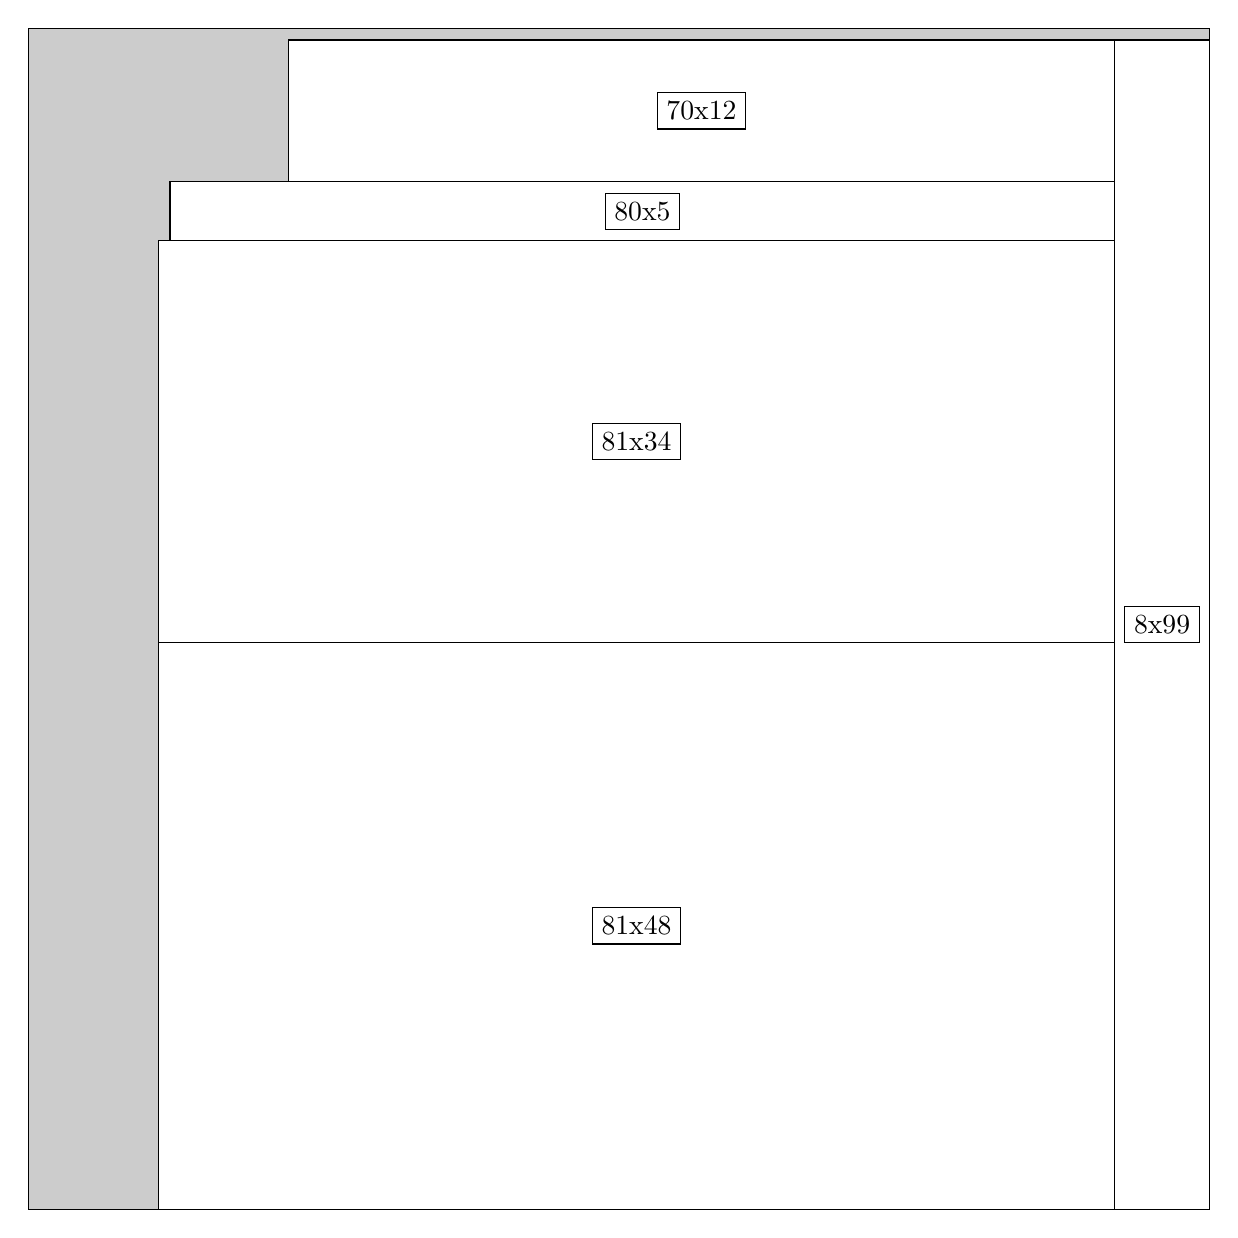
\begin{tikzpicture}[shorten >=1pt,scale=1.0,every node/.style={scale=1.0},->]
\tikzstyle{vertex}=[circle,fill=black!25,minimum size=14pt,inner sep=0pt]
\filldraw[fill=gray!40!white, draw=black] (0,0) rectangle (15.0,15.0);
\foreach \name/\x/\y/\w/\h in {8x99/13.799999999999999/0.0/1.2/14.85,81x48/1.65/0.0/12.15/7.199999999999999,81x34/1.65/7.199999999999999/12.15/5.1,80x5/1.7999999999999998/12.299999999999999/12.0/0.75,70x12/3.3/13.049999999999999/10.5/1.7999999999999998}
\filldraw[fill=white!40!white, draw=black] (\x,\y) rectangle node[draw] (\name) {\name} ++(\w,\h);
\end{tikzpicture}


w =8 , h =99 , x =92 , y =0 , v =792
\par
w =81 , h =48 , x =11 , y =0 , v =3888
\par
w =81 , h =34 , x =11 , y =48 , v =2754
\par
w =80 , h =5 , x =12 , y =82 , v =400
\par
w =70 , h =12 , x =22 , y =87 , v =840
\par
\newpage


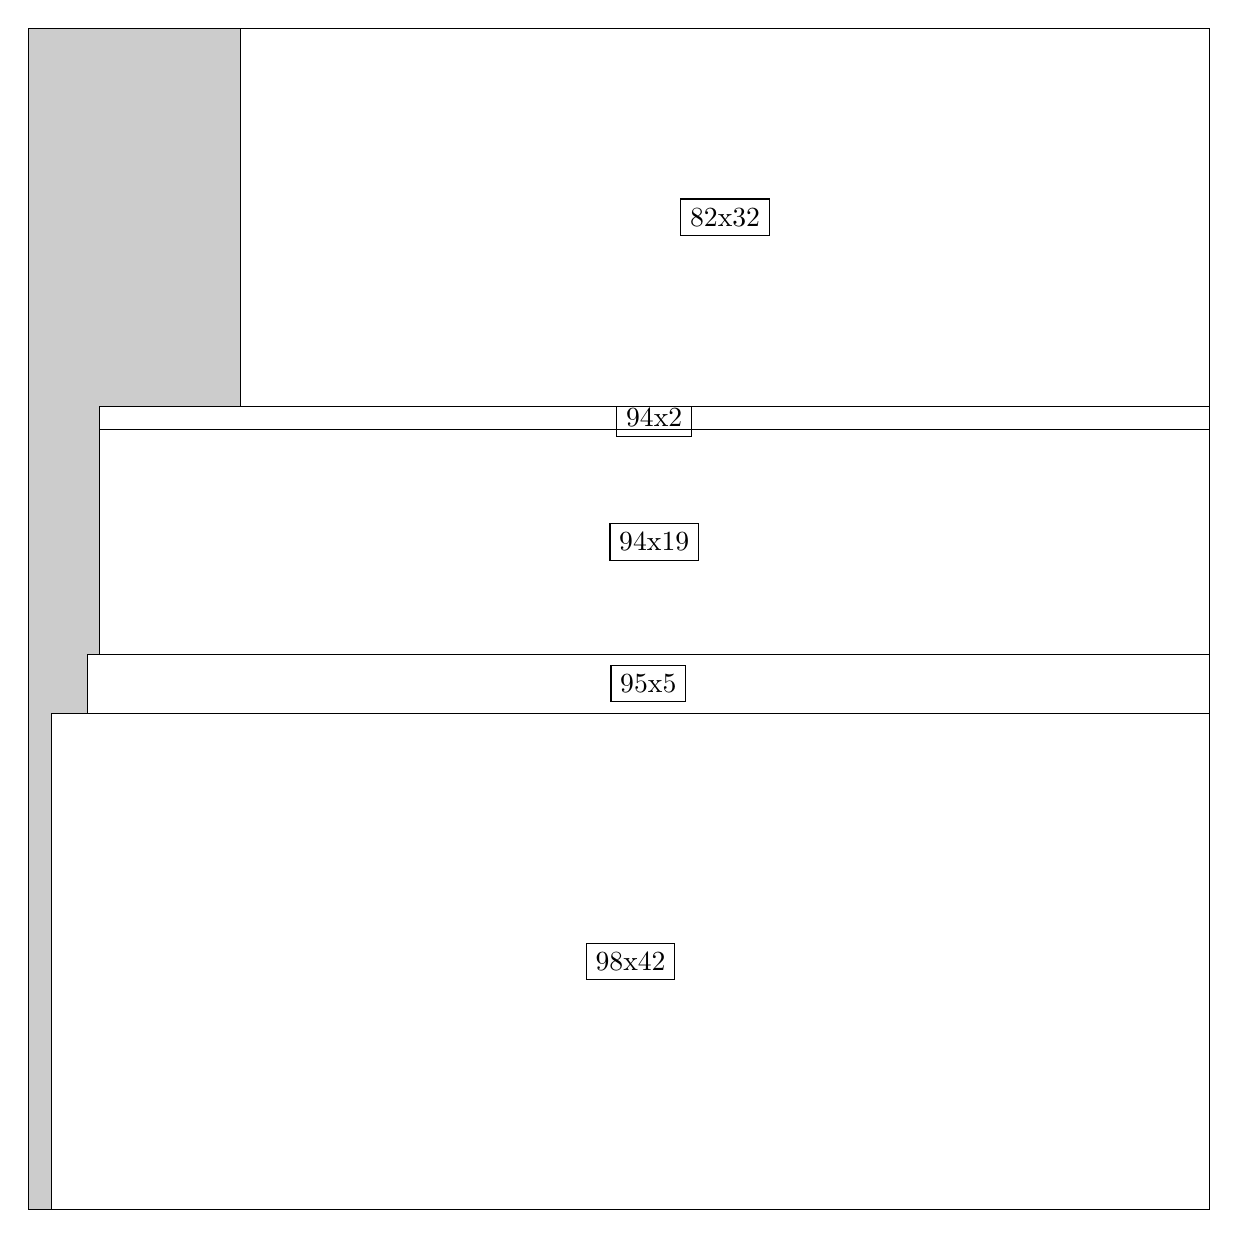
\begin{tikzpicture}[shorten >=1pt,scale=1.0,every node/.style={scale=1.0},->]
\tikzstyle{vertex}=[circle,fill=black!25,minimum size=14pt,inner sep=0pt]
\filldraw[fill=gray!40!white, draw=black] (0,0) rectangle (15.0,15.0);
\foreach \name/\x/\y/\w/\h in {98x42/0.3/0.0/14.7/6.3,95x5/0.75/6.3/14.25/0.75,94x19/0.8999999999999999/7.05/14.1/2.85,94x2/0.8999999999999999/9.9/14.1/0.3,82x32/2.6999999999999997/10.2/12.299999999999999/4.8}
\filldraw[fill=white!40!white, draw=black] (\x,\y) rectangle node[draw] (\name) {\name} ++(\w,\h);
\end{tikzpicture}


w =98 , h =42 , x =2 , y =0 , v =4116
\par
w =95 , h =5 , x =5 , y =42 , v =475
\par
w =94 , h =19 , x =6 , y =47 , v =1786
\par
w =94 , h =2 , x =6 , y =66 , v =188
\par
w =82 , h =32 , x =18 , y =68 , v =2624
\par
\newpage


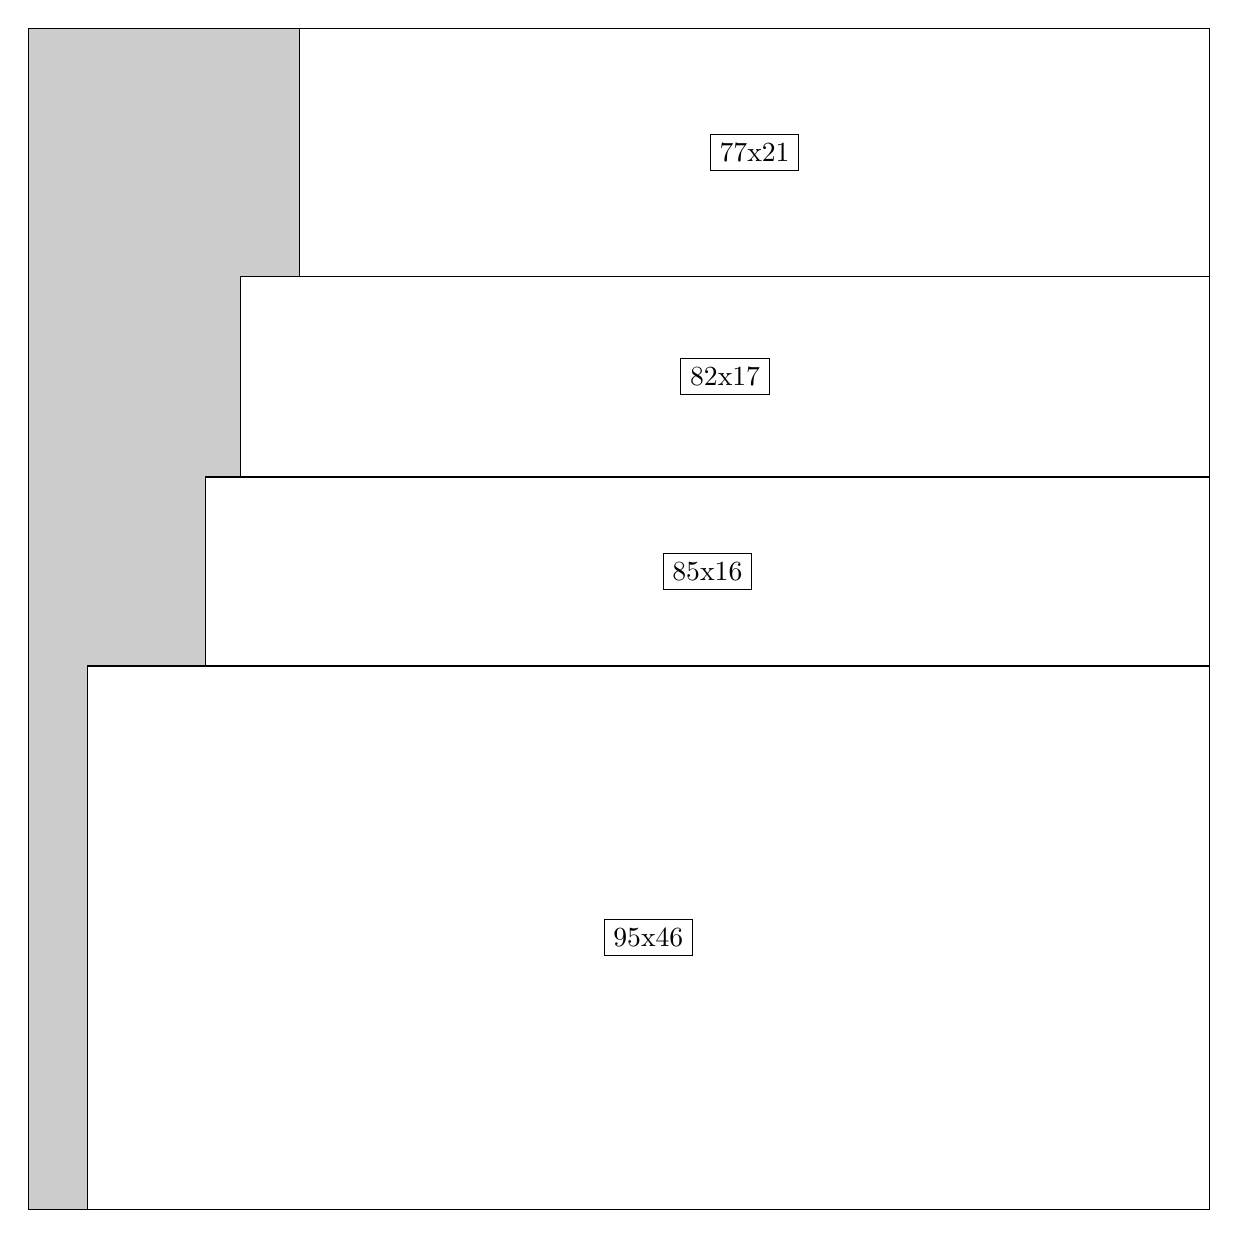
\begin{tikzpicture}[shorten >=1pt,scale=1.0,every node/.style={scale=1.0},->]
\tikzstyle{vertex}=[circle,fill=black!25,minimum size=14pt,inner sep=0pt]
\filldraw[fill=gray!40!white, draw=black] (0,0) rectangle (15.0,15.0);
\foreach \name/\x/\y/\w/\h in {95x46/0.75/0.0/14.25/6.8999999999999995,85x16/2.25/6.8999999999999995/12.75/2.4,82x17/2.6999999999999997/9.299999999999999/12.299999999999999/2.55,77x21/3.4499999999999997/11.85/11.549999999999999/3.15}
\filldraw[fill=white!40!white, draw=black] (\x,\y) rectangle node[draw] (\name) {\name} ++(\w,\h);
\end{tikzpicture}


w =95 , h =46 , x =5 , y =0 , v =4370
\par
w =85 , h =16 , x =15 , y =46 , v =1360
\par
w =82 , h =17 , x =18 , y =62 , v =1394
\par
w =77 , h =21 , x =23 , y =79 , v =1617
\par
\newpage


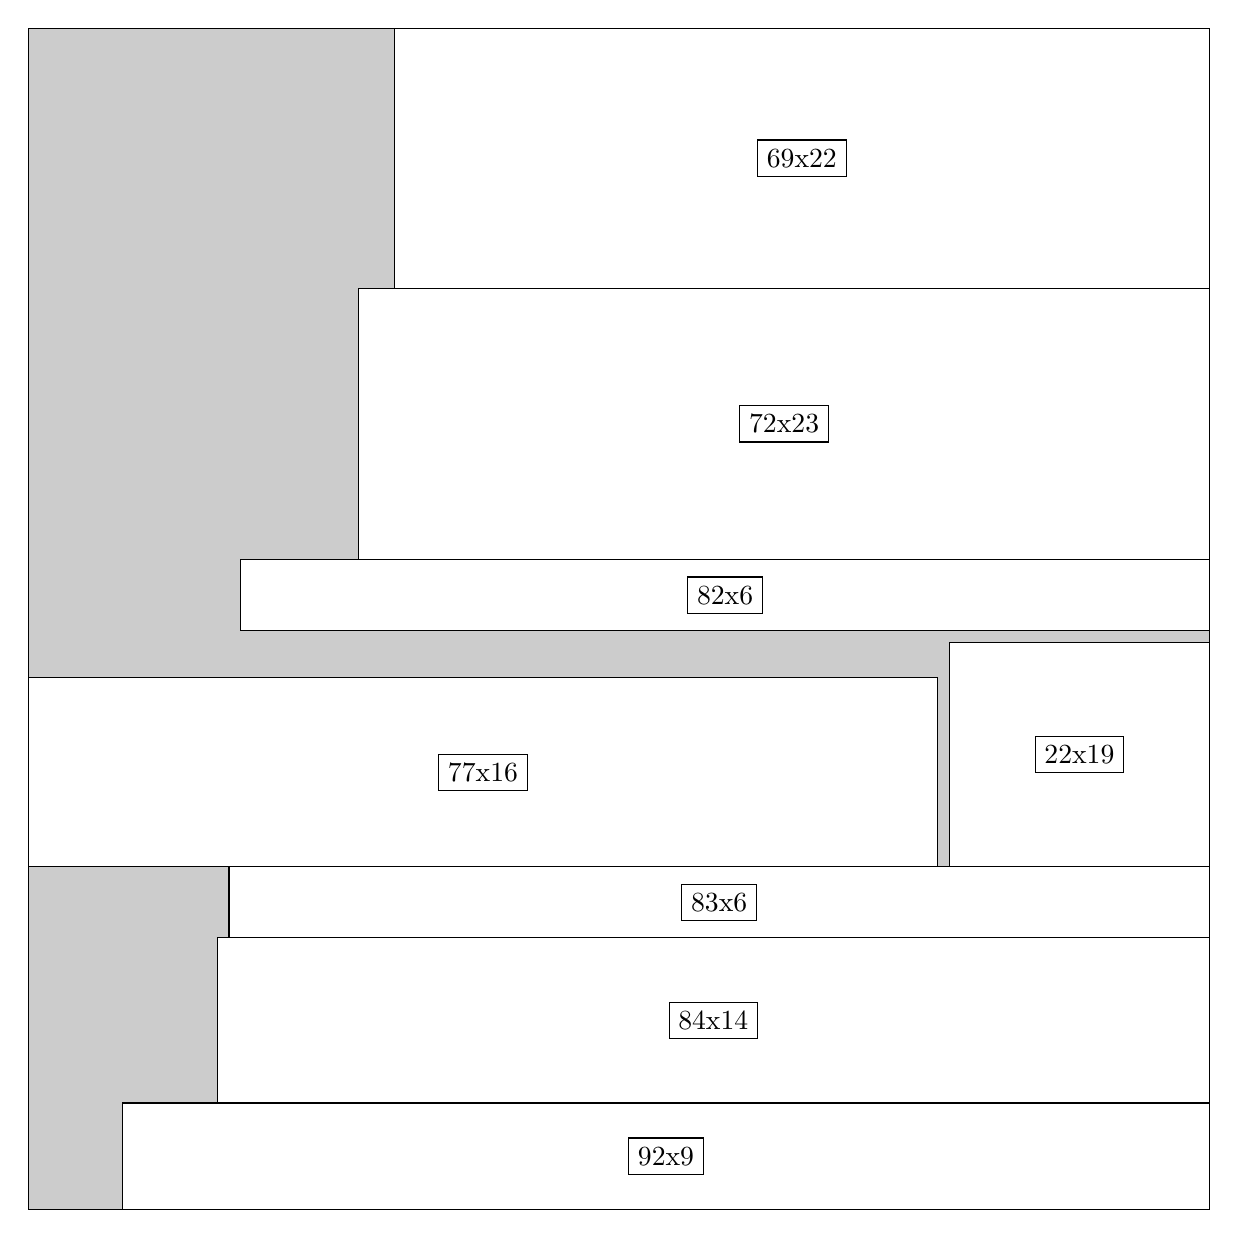
\begin{tikzpicture}[shorten >=1pt,scale=1.0,every node/.style={scale=1.0},->]
\tikzstyle{vertex}=[circle,fill=black!25,minimum size=14pt,inner sep=0pt]
\filldraw[fill=gray!40!white, draw=black] (0,0) rectangle (15.0,15.0);
\foreach \name/\x/\y/\w/\h in {92x9/1.2/0.0/13.799999999999999/1.3499999999999999,84x14/2.4/1.3499999999999999/12.6/2.1,83x6/2.55/3.4499999999999997/12.45/0.8999999999999999,22x19/11.7/4.35/3.3/2.85,77x16/0.0/4.35/11.549999999999999/2.4,82x6/2.6999999999999997/7.35/12.299999999999999/0.8999999999999999,72x23/4.2/8.25/10.799999999999999/3.4499999999999997,69x22/4.6499999999999995/11.7/10.35/3.3}
\filldraw[fill=white!40!white, draw=black] (\x,\y) rectangle node[draw] (\name) {\name} ++(\w,\h);
\end{tikzpicture}


w =92 , h =9 , x =8 , y =0 , v =828
\par
w =84 , h =14 , x =16 , y =9 , v =1176
\par
w =83 , h =6 , x =17 , y =23 , v =498
\par
w =22 , h =19 , x =78 , y =29 , v =418
\par
w =77 , h =16 , x =0 , y =29 , v =1232
\par
w =82 , h =6 , x =18 , y =49 , v =492
\par
w =72 , h =23 , x =28 , y =55 , v =1656
\par
w =69 , h =22 , x =31 , y =78 , v =1518
\par
\newpage


\end{document}